\documentclass{beamer}
\mode<presentation>
\usepackage{amsmath}
\usepackage{amssymb}
%\usepackage{advdate}
\usepackage{adjustbox}
\usepackage{subcaption}
\usepackage{enumitem}
\usepackage{multicol}
\usepackage{mathtools}
\usepackage{listings}
\usepackage{physics}
\usepackage{url}
\def\UrlBreaks{\do\/\do-}
\usetheme{Boadilla}
\usecolortheme{lily}
\setbeamertemplate{footline}
{
  \leavevmode%
  \hbox{%
  \begin{beamercolorbox}[wd=\paperwidth,ht=2.25ex,dp=1ex,right]{author in head/foot}%
    \insertframenumber{} / \inserttotalframenumber\hspace*{2ex} 
  \end{beamercolorbox}}%
  \vskip0pt%
}

\providecommand{\nCr}[2]{\,^{#1}C_{#2}} % nCr
\providecommand{\nPr}[2]{\,^{#1}P_{#2}} % nPr
\providecommand{\mbf}{\mathbf}
\providecommand{\pr}[1]{\ensuremath{\Pr\left(#1\right)}}
\providecommand{\qfunc}[1]{\ensuremath{Q\left(#1\right)}}
\providecommand{\sbrak}[1]{\ensuremath{{}\left[#1\right]}}
\providecommand{\lsbrak}[1]{\ensuremath{{}\left[#1\right.}}
\providecommand{\rsbrak}[1]{\ensuremath{{}\left.#1\right]}}
\providecommand{\brak}[1]{\ensuremath{\left(#1\right)}}
\providecommand{\lbrak}[1]{\ensuremath{\left(#1\right.}}
\providecommand{\rbrak}[1]{\ensuremath{\left.#1\right)}}
\providecommand{\cbrak}[1]{\ensuremath{\left\{#1\right\}}}
\providecommand{\lcbrak}[1]{\ensuremath{\left\{#1\right.}}
\providecommand{\rcbrak}[1]{\ensuremath{\left.#1\right\}}}
\theoremstyle{remark}
\newtheorem{rem}{Remark}
\newcommand{\sgn}{\mathop{\mathrm{sgn}}}
\providecommand{\abs}[1]{\left\vert#1\right\vert}
\providecommand{\res}[1]{\Res\displaylimits_{#1}} 
\providecommand{\norm}[1]{\lVert#1\rVert}
\providecommand{\mtx}[1]{\mathbf{#1}}
\providecommand{\mean}[1]{E\left[ #1 \right]}
\providecommand{\fourier}{\overset{\mathcal{F}}{ \rightleftharpoons}}
%\providecommand{\hilbert}{\overset{\mathcal{H}}{ \rightleftharpoons}}
\providecommand{\system}{\overset{\mathcal{H}}{ \longleftrightarrow}}
	%\newcommand{\solution}[2]{\textbf{Solution:}{#1}}
%\newcommand{\solution}{\noindent \textbf{Solution: }}
\providecommand{\dec}[2]{\ensuremath{\overset{#1}{\underset{#2}{\gtrless}}}}
\newcommand{\myvec}[1]{\ensuremath{\begin{pmatrix}#1\end{pmatrix}}}
\let\vec\mathbf

\lstset{
%language=C,
frame=single, 
breaklines=true,
columns=fullflexible
}

\numberwithin{equation}{section}

\lstset{
  language=Python,
  basicstyle=\ttfamily\small,
  keywordstyle=\color{blue},
  stringstyle=\color{orange},
  numbers=left,
  numberstyle=\tiny\color{gray},
  breaklines=true,
  showstringspaces=false
}

\title{Problem 2.4.8}
\author{ee25btech11018-Darisy Sreetej}

\date{\today} 
\begin{document}

\begin{frame}
\titlepage
\end{frame}

\section{Problem}
\begin{frame}
\frametitle{Problem Statement}
%
Find a unit vector perpendicular to each of the vectors $\myvec{\vec{a}+\vec{b}}$ and $\myvec{\vec{a}+\vec{b}}$ where, $\vec{a} = \hat{i} + \hat{j} + \hat{k}$ and $\vec{b} = \hat{i} + 2\hat{j} + 3\hat{k} $ is
\end{frame}
%\subsection{Literature}
\section{Solution}
\begin{frame}
\frametitle{Solution}
\setcounter{section}{1}
%\framesubtitle{Literature}
Let the desired vector be $\vec{x}$.
Then,
$\vec{x}=\myvec{x_1 \\
x_2\\
x_3}$
\begin{align}
\myvec{\vec{a}+\vec{b}}=\myvec{\vec{a}&\vec{b}}\myvec{1\\1}
\end{align}
\begin{align}
\myvec{\vec{a}-\vec{b}}=\myvec{\vec{a}&\vec{b}}\myvec{1\\-1}
\end{align}
According to the given question ,
\begin{align}
    \therefore \myvec{\vec{a}+\vec{b}&\vec{a}-\vec{b}}^T\vec{x}=0
\end{align}
(0.4) can be expressed as
\begin{align}
    \cbrak{{\myvec{\vec{a}&\vec{b}}\myvec{1&&1\\1&&-1}}}^T\vec{x}=0
    \end{align}
    \begin{align}
       \myvec{1&&1\\1&&-1}^T \myvec{\vec{a}&\vec{b}}^T\vec{x}=0
    \end{align}
\end{frame}
\begin{frame}
\frametitle{Solution}
\begin{align}
         \myvec{1&&1\\1&&-1}\myvec{1&&1\\1&&-1}^T \myvec{\vec{a}&\vec{b}}^T\vec{x}=0
    \end{align}
    or,
    \begin{align}
        \myvec{\vec{a}&\vec{b}}^T\vec{x}=0
    \end{align}
which can be expressed as 
\begin{align}
    \myvec{1&&1&&1\\1&&2&&3}
    \xleftrightarrow{ R_2 = R_2 - R_1}
    \myvec{1&&1&&1\\0&&1&&2}
    \end{align}
    and
    \begin{align}
     \myvec{1&&1&&1\\1&&2&&3}
    \xleftrightarrow{ R_2 = R_2 - 2R_1}
    \myvec{1&&1&&1\\-1&&0&&1}
\end{align}
\end{frame}
\begin{frame}
\frametitle{Solution}
yielding,
\begin{align}
    x_2+2x_3=0\\
    -x_1+x_3=0
\end{align}
\begin{align}
    \vec{x}=x_3\myvec{1\\-2\\1}
\end{align}
The unit vector is 
\begin{align}
      \vec{x}=\frac{1}{\sqrt{6}}\myvec{1\\-2\\1}
\end{align}
As we know that the vector can be in both the directions i.e, into and out of the plane containing $\vec{a}$ and $\vec{b}$, so the vector perpendicular to vectors $\vec{a}$ and $\vec{b}$ would be $\pm\;(\vec{a} \times \vec{b})$.

\end{frame}
\begin{frame}
\frametitle{Solution}
Therefore, the desired output is
\begin{align}
    \vec{x}=\pm\frac{1}{\sqrt{6}}\myvec{1\\-2\\1}
\end{align}
\end{frame}

\begin{frame}[fragile]
\frametitle{Plot-Graph}

\begin{figure}[h!]
   \centering
   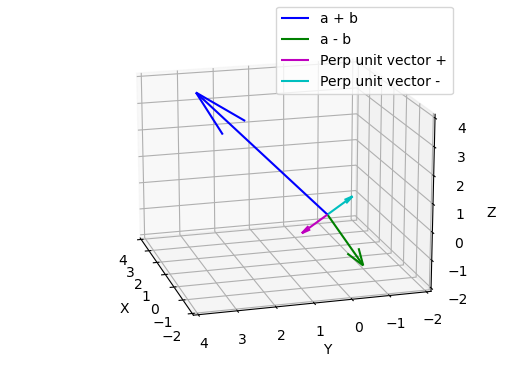
\includegraphics[width=0.7\columnwidth]{figs/fig.png}
	\caption{}
   \label{stemplot}
\end{figure}
\end{frame}

\section{C Code}
\begin{frame}[fragile]
\frametitle{C Code for finding vectors}
\begin{lstlisting}[language=C]
void get_unit_vectors(double result[6]) {
    double a[3] = {1, 1, 1};
    double b[3] = {1, 2, 3};
    double sum[3], cross[3], mag;
    int i;
    for(i=0;i<3;i++) sum[i]=a[i]+b[i];
    cross[0] = sum[1]*b[2] - sum[2]*b[1];
    cross[1] = sum[2]*b[0] - sum[0]*b[2];
    cross[2] = sum[0]*b[1] - sum[1]*b[0];
    mag = sqrt(cross[0]*cross[0] + cross[1]*cross[1] + cross[2]*cross[2]);
    if (mag == 0.0) {
        for(i=0;i<6;i++) result[i]=-999; // error
        return;
    }
    for(i=0;i<3;i++) {
        result[i] = cross[i]/mag;     // positive unit vector
        result[i+3] = -cross[i]/mag;  // negative unit vector }   
}
    \end{lstlisting}
\end{frame}
\section{Python Code}
\begin{frame}[fragile]
\frametitle{Calling C Function}
\begin{lstlisting}[language=Python]
import ctypes
import numpy as np

# Load the shared library
lib = ctypes.CDLL('./unitvector.so')

# Define argument and return types
lib.get_unit_vectors.argtypes = [ctypes.POINTER(ctypes.c_double)]
lib.get_unit_vectors.restype = None

# Create an array of 6 doubles to store results from C
result_arr = (ctypes.c_double * 6)()

# Call the C function
lib.get_unit_vectors(result_arr)

# Convert the result to numpy array for easy handling
results = np.array(result_arr)
\end{lstlisting}
\end{frame}

\begin{frame}[fragile]
\frametitle{Calling C Function}
\begin{lstlisting}[language=Python]

if results[0] == -999:
    print("Error: vectors are parallel or no unique perpendicular vector.")
else:
    print(f"Positive unit vector: ({results[0]:.3f}, {results[1]:.3f}, {results[2]:.3f})")
    print(f"Negative unit vector: ({results[3]:.3f}, {results[4]:.3f}, {results[5]:.3f})")

\end{lstlisting}
\end{frame}

\begin{frame}[fragile]
\frametitle{Python Code for Plotting}
\begin{lstlisting}[language=Python]
import numpy as np
import matplotlib.pyplot as plt
from mpl_toolkits.mplot3d import Axes3D

# Given vectors
a = np.array([1, 1, 1])
b = np.array([1, 2, 3])
sum_vec = a + b
diff_vec = a - b

# Cross product to find perpendicular unit vector to both (a+b) and (a-b)
cross = np.cross(sum_vec, diff_vec)
mag = np.linalg.norm(cross)

if mag == 0:
    raise ValueError("Vectors are parallel; no unique perpendicular vector.")

\end{lstlisting}
\end{frame}

\begin{frame}[fragile]
\frametitle{Python Code for Plotting}
\begin{lstlisting}[language=Python]
unit_pos = cross / mag
unit_neg = -unit_pos

# Plotting
fig = plt.figure()
ax = fig.add_subplot(111, projection='3d')

origin = np.zeros(3)

# Plot vectors a+b and a-b
ax.quiver(*origin, *sum_vec, color='b', label="a + b")
ax.quiver(*origin, *diff_vec, color='g', label="a - b")

# Plot positive and negative perpendicular unit vectors
ax.quiver(*origin, *unit_pos, color='m', label="Perp unit vector +")
ax.quiver(*origin, *unit_neg, color='c', label="Perp unit vector -")

\end{lstlisting}
\end{frame}

\begin{frame}[fragile]
\frametitle{Python Code for Plotting}
\begin{lstlisting}[language=Python]
# Set limits and labels
ax.set_xlim([min(0, -2), max(4, 4)])
ax.set_ylim([min(0, -2), max(4, 4)])
ax.set_zlim([min(0, -2), max(4, 4)])
ax.set_xlabel('X')
ax.set_ylabel('Y')
ax.set_zlabel('Z')
ax.legend()

plt.title('3D plot of (a+b), (a-b) and perpendicular unit vectors')
plt.show()
\end{lstlisting}
\end{frame}

\end{document}